% LaTeX template for MLSP papers. To be used with:
%   * mlspconf.sty - ICASSP/ICIP LaTeX style file adapted for MLSP, and
%   * IEEEbib.bst - IEEE bibliography style file.
% --------------------------------------------------------------------------
\documentclass{article}
\usepackage{amsmath,graphicx,mlspconf}

% Copyright notices.
% ------------------
% Select one of the four copyright notices below. Only required for the camera-ready paper submission.
% 
% * For papers in which all authors are employed by the US government:
\copyrightnotice{U.S.\ Government work not protected by U.S.\ copyright}

% * For papers in which all authors are employed by a Crown government (UK, Canada, and Australia):
\copyrightnotice{979-8-3503-2411-2/23/\$31.00 {\copyright}2023 Crown}

% * For papers in which all authors are employed by the European Union:
\copyrightnotice{979-8-3503-2411-2/23/\$31.00 {\copyright}2023 European Union}

% * For all other papers:
\copyrightnotice{979-8-3503-2411-2/23/\$31.00 {\copyright}2023 IEEE}

% Header
\toappear{2023 IEEE International Workshop on Machine Learning for Signal Processing, Sept.\ 17--20, 2023, Rome, Italy}

% Example definitions.
% --------------------
%\def\x{{\mathbf x}}
%\def\L{{\cal L}}

% Title.
% ------
\title{A Probabilistic Semi-Supervised Approach with Triplet Markov Chains}
%
% Double-blind peer review.
% -------------------------
% Anonymize your paper for the double-blind peer-review process using the 
% following author and affiliation.
\name{Anonymous\thanks{Anonymous.}}
\address{Anonymous}

% Single address.
% ---------------
%\name{Author(s) Name(s)\thanks{Thanks to XYZ agency for funding.}}
%\address{Author Affiliation(s)}

% For example:
% ------------
%\address{%
%    School \\
%    Department \\
%    Address
%}
%
% Two addresses.
% --------------
%\twoauthors{%
%    A. Author-one, B. Author-two\sthanks{Thanks to XYZ agency for funding.}
%}{%
%    School A-B \\
%    Department A-B \\
%    Address A-B \\
%    Email A-B
%}{%
%   C. Author-three, D. Author-four\sthanks{The fourth author performed the work while at ...}
%}{%
%    School C-D \\
%    Department C-D \\
%    Address C-D \\
%    Email C-D
%}
% 
% Two or more addresses (alternative form).
% -----------------------------------------
% If you need to list more than 2 authors or the option for two options above 
% produces a poor author block, please use the following structure:
%\name{%
%    Author Name$^{\star \dagger}$%
%    \qquad Author Name$^{\star}$%
%    \qquad Author Name$^{\dagger}$\thanks{Thanks to XYZ agency for funding.}%
%}
%\address{%
%    $^{\star}$ Affiliation Number One \\%
%    $^{\dagger}$ Affiliation Number Two%
%}

% -----------------------------------------
% Packages
\usepackage{graphicx,xcolor,verbatim}
\usepackage{amsfonts}
\usepackage{multirow}
\usepackage{amsmath}
\usepackage{todonotes}
\usepackage[export]{adjustbox}
\usepackage{xcolor}

% -----------------------------------------
% Notations
\DeclareMathOperator*{\argmax}{arg\,max}
\def\x{{\mathbf x}}
\def\z{{\mathbf z}}
\def\y{{\mathbf y}}
\def\yl{{\mathbf y}_{T^{\mathcal{L}}}}
\def\yu{{\mathbf y}_{T^{\mathcal{U}}}}

\def\h{{\mathbf h}}
\def\hh{{\mathbf h'}}
\def\L{{\mathcal L}}
\def\N{{\mathcal N}}
\def\Ber{{\mathcal Ber}}
\def\E{{\mathbb{E}}}
\def\p{p_{\theta}}
\def\q{q_\phi}
\def\Q{\tilde{Q}}
\def\hh{\overline{h}}
\def\D{\mathcal{D}}
\def\L{\mathcal{L}}
\def\U{\mathcal{U}}
\def\Du{\mathcal{D}^{\mathcal{U}}}
\def\Dl{\mathcal{D}^{\mathcal{L}}}

%\newcommand{\argmin}{\mathop{\mathrm{arg\,min}}
\def\dkl{\mathrm{D}_{\mathrm{KL}}}
\def\argmin{\underset{q\in \mathcal{Q}}{\mathrm{arg\,min}}}
\newcommand{\katyN}[1]{\todo[inline,color=pink]{#1 --- Katy}}
\newcommand{\katy}[1]{\todo[size=\tiny,color=pink]{#1  \hfill --- Kat}}
\newcommand{\observation}[1]{\todo[size=\tiny,color=orange]{#1  \hfill --- obs}}
% \newcommand{\corrections}[2]{\stcyan{#1}~\cyan{#2}}
%===============================
\newtheorem{example}{Example}
\newtheorem{remark}{Remark}
\newcommand{\cfbox}[2]{%
    \colorlet{currentcolor}{.}%
    {\color{#1}%
    \fbox{\color{currentcolor}#2}}%
}
%===============================
% -----------------------------------------
% -----------------------------------------
% -----------------------------------------





\begin{document}
%\ninept

\maketitle

\begin{abstract}
% The abstract should contain about 100 to 150 words,
In this article, xxx
\end{abstract}
%
\begin{keywords}
Generative Models; Variational Inference; Semi-Supervised Learning; Triplet Markov Chains.
\end{keywords}
%
\section{Introduction}
\label{sec:intro}
Let $\x_T=(x_{0}, \dots, x_{T})$ and $\z_T=(z_{0}, \dots, z_{T})$  be two
sequences of observed and latent  random variables (r.v.), respectively, 
where  $x_t \in \mathbb{R}^{d_x}$ and $z_t \in \mathbb{R}^{d_z}$. 
We also define a  third process of discrete values $\y_T=(y_{0}, \dots,\; y_{T})$, 
where $y_t \in \Omega=\{\omega_1,\dots,\omega_C\}$.
As far as notations are concerned, we do not distinguish r.v. and their realizations.

\subsection{Semi-Supervised learning}
Sequential data is characterized by a temporal ordering of observations. 
It is commonly used in many fields, such as speech recognition XX, 
natural language processing XX, and activity recognition XX, etc. 
Labeled sequential data is sequential data that is annotated with labels
that indicate the meaning or class of each observation.
These labels are essential for many applications, such as supervised classification, 
anomaly detection, and clustering.
However, in many real-world applications, it is expensive or impossible to obtain
labels for the entire sequence due to various reasons such as the high cost of
labeling, the lack of expertise, or the lack of time. 
In such cases, partially labeled sequential data, which only has labels 
for some of the observations, can be used instead.


Partially labeled sequential data presents a challenging problem for machine 
learning algorithms XX because they need to leverage both the labeled and 
unlabeled parts of the data to learn a good model. 
This problem is known as semi-supervised learning, and it has been studied 
extensively in the machine learning community,  it can be handle using
different techniques XXX.
% transfer learning XX, 
% graph-based methods XX,  generative models XX, among others.
In particular, generative models are a popular approach for semi-supervised learning, 
as they allow the incorporation of prior knowledge about the data distribution.
In the case of sequential data, probabilistic generative models can be used to
model the underlying distribution of the data and generate new samples,
make predictions outcomes, and estimate missing or unobserved data. 



One approach for semi-supervised learning is to design a latent variable 
generative model, which can represent complex temporal relations, 
and then propose a variational method for learning and inference XXX. 
Some popular examples of generative models  include 
Hidden Markov Chains (HMCs)~\cite{rabiner1989tutorial} and  Pairwise Markov
Chains (PMCs) \cite{morales2021variational,wp-pami} which are used for modeling sequential data and 
are based on latent variables.
However, they have not been adapted to the case of partially labeled 
sequential data... \observation{I'm not sure}. 

In this article, we proposea more general generative model called 
Triplet Markov Chain (TMC)~\cite{wp-cras-chaines3,pieczynski2005triplet} 


%  In a HMC, the sequence  $\z_T$ is a Markov chain and given $\z_T$, 
%  the observations $x_t$ are independent 
% and , given on $\Z_T$, the distribution of $x_t$ only depends 
% on the corresponding $z_t$.
% In other words, $\p(\z_K,\x_K)$ satisfies
% \begin{equation}
% \label{hmc}
%  \p(\z_T,\x_T)=\p(z_0)\prod_{t=1}^T \p(z_t|z_{t-1}) \prod_{t=0}^T \p(x_t|z_{t}) \text{,} 
% \end{equation}


% Ideas
%  The introduction of a continuous latent process $\z_T$ is interesting from a modeling point of view

\subsection{Scope of the paper}

Since  only a subset of the observations has corresponding labels,  
the sequence of labels can be expressed as  $\y_T  = \yl \cup \yu$,  
where  $\yl = \{y_t\}_{t\in \L}$  and $\yu = \{y_t\}_{t\in \U}$ are the sets
of observed labels and unobserved (hidden) labels, respectively; and $\mathcal{L}$ and 
$\mathcal{U}$ are the set of labeled and unlabeled time steps, respectively. 



In this article, our interest is to present a general generative model for 
semi-supervised learning,  based on latent r.v. which is defined by a joint 
distribution $\p(\x_T, \y_T, \z_T)$ and provides learning from the observations 
$\x_T$ and the observed labels $\yl$,  since the distribution reads 

\begin{align}
    \label{eq:jointTMC}
    \p(\x_T, \yl) =  \sum_{y_t\in \yu} \int  \p(\x_T, \y_T,\z_T) {\rm d}\z_T \text{.}
\end{align}

Our model is based on the TMC \cite{wp-cras-chaines3,pieczynski2005triplet} which
relies on the assumption that the  triplet $(z_t, y_t, x_t)_{t \geq 0}$ 
is a Markov chain with transition $p(z_t, y_t, x_t|z_{t-1},y_{t-1},x_{t-1})$.


% First, $(\x_T, \y_T, \z_T)$ are described by a parameterized distribution
% $\p(\x_T, \y_T,  \z_T)$ which allows to model the unknown distribution 
% $p(\x_T, \y_T, \z_T)$. Next, the set of parameters $\theta$ is estimated 
% from the realizations   $\x_T$ and the observed labels $\yl$. 





\section{Proposed method}
\label{sec:ourmethod}
This section presents a review of variational Bayesian inference and its
application to general Triplet Markov Chains for semi-supervised learning.

\subsection{Background: Variational Inference}
\label{subsec:varinf}
The aim is to estimate the parameter $\theta$ from a realization $\x_T$. 
A popular estimate is the Maximum-Likelihood (ML) estimate 
$\hat{\theta}=\argmax_{\theta} \p(\x_T)$
due to its statistical properties \cite{White-MLE, Douc-ML-MIS}.
However, a direct maximization of $\p(\x_T)$ is not always possible, particularly in
models with latent variables where the likelihood
$\p(\x_T)=\int \p(\x_T,\z_T) {\rm d}\z_T$ may be not computable. 
% On the other hand, variational inference is a powerful tool for approximating 
% complex posterior $\p(\z_T|\x_T)$ distributions in probabilistic models. 
% Because the likelihood is not computable in the general case, 
In the variational inference framework, a variational lower bound called evidence lower bound 
(ELBO) on the log-likelihood  is optimized in order to estimate the parameters $\theta$.
This variational lower bound relies on the introduction of a parameterized 
variational distribution $\q(\z_T|\x_T)$, which is parameterized by a set of parameters $\phi$, 
and it is given by: 

\vspace{-0.2cm}
\begin{align}
&\log(\p(\x_T)) \geq \Q(\theta,\phi) \text{,} \nonumber \\
\label{eq:elbo}
&\Q(\theta,\phi) = - \int \log \left(\frac{\q(\z_T|\x_T)}{\p(\x_T,\z_T)}\right) \q(\z_T|\x_T) {\rm d} \z_T \text{.}
\end{align}
\vspace{-0.3cm}

Equality holds if $\q(\z_T\x_T)= \p(\z_T|\x_T)$.
When the posterior distribution $\p(\z_T|\x_T)$ is  computable, the alternating 
maximization w.r.t. $\theta$ and $\q$  of the ELBO, $\Q(\theta,\phi)$,
coincides with the EM algorithm \cite{variational-EM}. 

Variational inference consists in maximizing $Q(\theta,\phi)$ 
with respect to $(\theta,\phi)$ for a given class of distributions $\q$. 
The choice of the variational distribution $\q(\z_T|\x_T)$ is important; 
$\q(\z_T|\x_T)$ should be close to $\p(\z_T|\x_T)$ but should also
be chosen in a such way that the associated ELBO can be exactly computed or 
easily approximated while remaining differentiable w.r.t. $(\theta,\phi)$. 
A simple way to approximate $\Q(\theta,\phi)$ is by using the reparametrization 
trick~\cite{kingma2013auto} which consists in chosing a parametric
distribution $\q(\z_T|\x_T)$ such that a sample $\z_T^{(i)} \sim q(\z_T|\x_T)$ can
be written as a differentiable function of $\phi$.

It remains to choose a variational distribution $\q(\z_T|\x_T)$.
One popular strategy is to use distributions from a mean-field variational 
distribution which factorizes as  $\q(\z_T|\x_T)=q(z_0|\x_T) \prod_{t=1}^t
\q(z_t|z_{0:t-1},\x_T)$.

\subsection{Semi-supervised Variational Inference for TMC}
\label{subsec:vi_tmc}

The TMC  is a direct generalization of PMC and HMC to the case where the

In this article, we present the TMC as a generative model which will be used 
% \katy{Complete this paragraph}

The distribution $p_{\theta}(\x_T, \y_T, \z_T)$ reads
\begin{align}
\label{eq:TMC}
&p_{\theta}(z_0,y_0, x_0) \prod_{t=1}^T  p_{\theta}(z_t, y_t, x_t|z_{t-1},y_{t-1}, x_{t-1})   \text{.}
\end{align}


Since  only a subset of labels is observed $\yl$, the set of unobserved 
labels $\yu$ is treated as latent variables and variational inference 
involves finding a lower bound on the marginal likelihood of the observed data $\x_T$ and $\yl$.
The variational lower bound is given by: 
% So the latent variables $\z_T$ and $\yu$ are unobserved variables that are not 
% directly measurable or observable, but are inferred from the observed data  $\x_T$ and $\yl$. 
\begin{align}
    \label{eq:elbo_semi_tmc}
    \log(\p(\x_T, \yl) )   \geq  & -  \int \sum_{\yu}  \q(\z_T, \yu|\x_T, \yl) \times \nonumber \\ 
    & \quad \quad  \log \left(\frac{\q(\z_T,\yu  |\x_T)}{\p(\z_T,\y_T, \x_T)}\right)  {\rm d} \z_T \nonumber \\
    & =  Q(\theta,\phi) \text{,}  
\end{align}
where $\phi$ denotes the parameters of the variational distribution 
$\q(\z_T,\yu|\x_T, \yl)$.

Since our model has both discrete and continuous latent variables, 
the approximation of the ELBO in Eq.~\eqref{eq:elbo_semi_tmc} becomes more complex.
To that end,  we can use the Gumbel-Softmax (G-S) 
trick~\cite{maddison2016concrete, jang2016categorical} and the reparametrization
trick~\cite{kingma2013auto} to approximate $Q(\theta,\phi)$ simustaneously.
For the continuous latent variables $\z_T$, the reparametrization 
trick introduced in section \ref{subsec:varinf} is still valid.
On the other hand, for the discrete latent variables $\yu$, 
the G-S trick enables to obtain a differentiable approximation to the discrete
categorical distribution. 

It remains to choose a factorization of the variational distribution
$\q(\z_T, \yu| \x_T, \yl)$, which is a crucial step in variational inference.
Different models can be obtained by choosing different factorizations 
of the variational distribution, which will be discussed 
in the next section \ref{subsec:particular_cases}. For example, we can first consider  
$\q(\z_T, \yu| \x_T, \yl) =  \q(\z_T| \x_T, \y_T ) \q(\yu| \x_T, \yl )$ 
and then consider a mean-field variational distribution.



% The computational complexity of using ELBO with both discrete and continuous 
% latent variables depends on the specific model and the size of the data. 
% In general, the Gumbel-Softmax trick involves sampling from a Gumbel
% distribution and applying a softmax function, which tends to be 
% computationally expensive. However, recent advances in hardware and 
% software have made such calculations feasible and efficient.


% \katy{I think we should add a paragraph here to explain what we do in the case
% of y is missing, we replace it by a sample .... }

\subsection{Particular cases of the TMC}
\label{subsec:particular_cases}
The choice of the factorization of the transition distribution 
$\p(z_t, y_t, x_t|z_{t-1},y_{t-1}, x_{t-1})$  has an impact on the
performance of the model for a specific task (classification, prediction,
detection or generation). 
The goal of this section is to present particular cases of our proposed TMC model
by choosing different factorizations of the transition and 
variational distribution.
For the sake of clarity, let us now denote the triplet $v_t=(x_t,z_t,y_t)$.

\subsubsection{VSL}
Variational Sequential Labelers model is a particular case of the TMC model
where the transition distribution is factorized as follows:
\begin{align}
\label{eq:vsl}
\p(v_t|v_{t-1}) \!= \!\p(y_t|z_t) \p(z_t|x_{t-1}, y_{t-1}) \p(x_t|z_t) \text{.}
\end{align}

In the case of SVRNN, the chosen variational distribution
$\q(\z_T, \yu| \x_T, \yl\!) \!=\!  \q(\z_T| \x_T, \yl\!) \q(\yu| \x_T, \z_T, \yl \!)$ 
is given by
\begin{align*}  
    \q(\z_T| \x_T, \yl ) =& \prod_{t=0}^T \q(z_t| \x_T) \\
    \q(\yu| \x_T, \z_T, \yl ) =& \prod_{t\in  \U}  \q(y_t| z_t)
\end{align*}
 
In particular, VLS considers $\q(y_t| z_t) =  \p(y_t| z_t)$.

\subsubsection{SVRNN}
A Semi-supervised Variational Recurrent Neural Network can be seen as an adapted
version of the TMC model where the latent variable $z_t$ is set as
 $(z'_t, h_t)$. The variable $z'_t$ is a stochastic latent variable 
and $h_t$ is deterministically given by $h_t = f_{\theta}(x_t, y_t, z'_t)$, 
where $f_{\theta}$ is a deterministic non-linear transition function. 
In ths case, the transition distribution is factorized as follows:
\begin{align}
\label{eq:svrnn}
\p(v_t|v_{t-1}\!) \!= \!\p(y_t|v_{t-1}\!) \p(z_t|y_t,\! v_{t-1}\!) \p(x_t|y_t,z_t,\!v_{t-1}\!) \text{.}
\end{align}

On the other hand, the chosen variational distribution 
$\q(\z_T, \yu| \x_T, \yl) =  \q(\z_T| \x_T, \y_T ) \q(\yu| \x_T, \yl )$  
factorizes as follows:
\begin{align*}
\q(\z_T| \x_T, \y_T ) =&  \q(z_0|\x_t, \y_t) \prod_{t=1}^T \q(z_t|\z_{t-1},\x_t, \y_t)  \\
\q(\yu| \x_T, \yl )=& \prod_{t\in  \U} \q(y_t|\y_{t-1}, \x_t) \text{,}
%\prod_{t\in  \U} \q(y_t|\y_{<t}, \x_t, \y_t) \text{,}
\end{align*}
% where $\y_{<t}$ refers to the set of unobserved labels with an index
% $t'\in  \U$  which satisfies $t'<t$.  



\subsubsection{mTMC}
Finally, we present the minimal TMC which  is a particular case of 
the TMC model  presented in~\cite{gangloff2023deep}
where 
the transition distribution is factorized as follows:
\begin{align}
    \label{eq:mTMC}
    \p(v_t|v_{t-1}) \!= \!\p(y_t|y_{t-1}) \p(z_t|z_{t-1}) \p(x_t|t_t,z_t) \text{.}
\end{align}
The variational distribution is chosen as in the SVRNN model.
\begin{align*}
    \q(\z_T| \x_T, \y_T ) =&  \q(z_0|\x_t, \y_t) \prod_{t=1}^T \q(z_t|\z_{t-1},\x_t, \y_t)  \\
    \q(\yu| \x_T, \yl )=& \prod_{t\in  \U} \q(y_t|\y_{t-1}, \x_t) \text{,}
\end{align*}

\section{Simulations}
\label{sec:simulation}
In this section, we present the results of the proposed models on
semi-supervised binary image segmentation. Our goal is to recover the segmentation of a binary image 
($\Omega=\{\omega_1,\omega_2\}$) from the noisy observations
$\x_T$ when a partially segmentation $\yl$ is available.

\subsection{Deep TMCs}
\label{subsec:deepTMC}
The set of parameters $(\theta, \phi)$  
%of the generating  and the variational distribution 
can be described by any differentiable flexible function $\psi(\cdot)$. 
In particular, we consider the case where the parameters are
produced by a (deep) neural network. 
% and call the resulting model a Deep TMC model.

Due to the different factorizations of the generating (resp. variational)
distributions, we consider a general notation
$\p(x_t | \cdot)$, $\p(z_t| \cdot)$ and $\p(y_t | \cdot)$ 
(resp. $\q(y_t | \cdot)$, $\q(z_t | \cdot)$) 
in order to avoid presenting a specific dependence between variables. 
These dependencies are specified for each model and are presented in the previous
Section~\ref{subsec:particular_cases}.
The general model is described by:
\begin{align}
    \p(v_t|v_{t-1}) &=  \p(x_t|\cdot) \p(z_t|\cdot)\p(y_t|\cdot) \nonumber\\
\label{eq:px}
    \p(x_t | \cdot) &= \N(x_t; \mu_{px, t}, {\rm diag}(\sigma_{px,t}) ) \\
\label{eq:pz}
    \p(z_t | \cdot) &= \N(x_t; \mu_{pz, t}, {\rm diag}(\sigma_{pz,t}) ) \\
\label{eq:py}
    \p(y_t | \cdot) &= \Ber(y_t;  \rho_{py,t}) \text{,}
\end{align}
where ${\rm diag(.)}$ denotes the diagonal matrix deduced from the values 
of $\sigma_{\cdot,t}$;   $[\mu_{\cdot,t}, \sigma_{\cdot,t}]$  and $\rho_{\cdot,t}$ denote 
the parameters of the Gaussian and Bernoulli distributions, respectively. 
Finally, the variational distribution is given by
\begin{align}
\label{eq:qz}
    \q(z_t | \cdot) &=  \N(z_t; \mu_{qz, t}, {\rm diag}(\sigma_{qz,t}) )\\  
\label{eq:qy}
    \q(y_t | \cdot) &=  \Ber(y_t;  \rho_{qy,t}) \text{,} 
\end{align}

The parameters $\theta = \{\mu_{pz,t}, \sigma_{pz,t}, \mu_{px,t}, \sigma_{px,t}, \rho_{py,t}\}$  
and $\phi = \{ \mu_{qz,t}, \sigma_{qz,t} , \rho_{qy,t}\}$ are derived from 
neural networks $(\psi_{px}, \psi_{pz}, \psi_{py})$ and 
$(\psi_{qz}, \psi_{qy})$, respectively.
Note that in the VLS model $\phi = \{ \mu_{qz,t}, \sigma_{qz,t} \}$ since 
the assumption $\q(y_t | z_t) = \p(y_t | z_t)$ is made. 
% \begin{example}
For example, we can consider the deep mTMC model where the parameters are given by:
\begin{align*}
% \label{eq:d1}
    &[\mu_{px,t}, \sigma_{px,t}]  = \psi_{px}(y_t, z_t)\\
% \label{eq:d2}
    &[\mu_{qz,t}, \sigma_{qz,t}] = \psi_{qz}( \z_{t-1},\x_t, \y_t )\text{, }\\
% \label{eq:d3}
    &[\mu_{pz,t}, \sigma_{pz,t}]  = \psi_{pz }(z_{t-1}), \\
% \label{eq:d4}
    &\rho_{py,t}  = \psi_{px}(y_{t-1})\\
% \label{eq:d5}
    &\rho_{qy,t}  = \psi_{qy}(\y_{t-1}, \x_t) \text{.}
\end{align*} 


% \end{example}


% \katy{Explicar la incorporacion de $h_t$ en el modelo SVRNN y como fue configurada
% en los otros modelos.}

\subsection{Experiments settings}
We consider the cattle-type and the camel-type images of the 
Binary Shape Database~\cite{binaryimg}.
The images are transformed into a $1$-D signal $\x_T$ with a Hilbert-Peano 
filling curve~\cite{sagan2012space}. 
They are next blurred with non-linear noises %($x_t|y_t,z_t$)
to highlight the ability, of the models presented
in Section~\ref{subsec:particular_cases}, to learn such a signal corruption.
In fact, the cattle-type image is blurred with a general stationary noise and 
the camel-type image is blurred with a stationary multiplicative noise 
(more details about generation are given in ~\cite{gangloff2023deep}).
On the other hand, the pixels $y_t \in \yl$ are randomly chosen. 
In particular, we consider that $60\%$ of pixels are labeled, 
the rest of pixels are considered as unobserved.



Each model was trained with stochastic gradient descent on the negative
associated ELBO using the Adam optimizer \cite{adam}. 
For each model,  $\psi_{\cdot}$ have two hidden layers using rectified linear units, 
with appropriate outputs (linear,  softplus and sigmoid).
Additionally, we match the total number of parameters of all models 
to be equal or close between them, so the number of hidden 
units, for each hidden layer, is different for each model.  
The SVRNN (resp. mTMC and VLS ) model 
has 22 (resp. 25  and 41) hidden units. 
% The SVRNN also considers a number
% of hidden units for the deterministic part of the model and it is equal to $XX$.



\subsection{Results}
\label{subsec:results}
The performance of the models is evaluated in terms of
the error rate (ER) of the reconstruction of the unobserved pixels. 

% Below is an example of how to insert images. Delete the ``\vspace'' line,
% uncomment the preceding line ``\centerline...'' and replace ``imageX.ps''
% with a suitable PostScript file name.
% -------------------------------------------------------------------------
\begin{figure}[htb]
    \begin{minipage}[b]{0.30\linewidth}
      \centering
      \centerline{
\includegraphics[width=\textwidth, cfbox=black 1pt 0pt]{ress/camel40/camel40.png}}
    %  \vspace{2.0cm}
      \centerline{Noisy image}\medskip
    \end{minipage}
    \hfill
    \begin{minipage}[b]{.30\linewidth}
      \centering
      \centerline{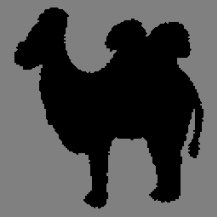
\includegraphics[width=\textwidth, cfbox=black 1pt 0pt]{ress/camel40/camel40_label.png}}
    %  \vspace{1.5cm}
      \centerline{100\% labeled }\medskip
    \end{minipage}
    \hfill
    \begin{minipage}[b]{0.30\linewidth}
      \centering
      \centerline{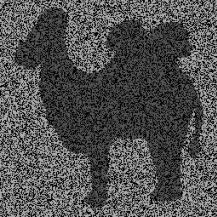
\includegraphics[width=\textwidth,cfbox=black 1pt 0pt]{ress/camel40/camel40_miss.png}}
    %  \vspace{1.5cm}
      \centerline{60\% labeled }\medskip
    \end{minipage}
    \\
    \begin{minipage}[b]{0.30\linewidth}
        \centering
        \centerline{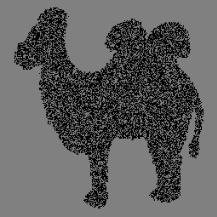
\includegraphics[width=\textwidth,cfbox=black 1pt 0pt]{ress/camel40/camel40_vsl.png}}
      %  \vspace{2.0cm}
        \centerline{VLS (41.84\%)}\medskip      \end{minipage}
      \hfill
      \begin{minipage}[b]{.30\linewidth}
        \centering
        \centerline{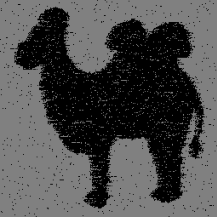
\includegraphics[width=\textwidth,cfbox=black 1pt 0pt]{ress/camel40/camel40_svrnn_2.png}}
      %  \vspace{1.5cm}
        \centerline{SVRNN (12.12\%)}\medskip
      \end{minipage}
      \hfill
      \begin{minipage}[b]{0.30\linewidth}
        \centering
        \centerline{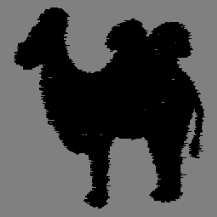
\includegraphics[width=\textwidth,cfbox=black 1pt 0pt]{ress/camel40/camel40_tmm_3.png}}
      %  \vspace{1.5cm}
        \centerline{mTMC (2.60\%)}\medskip
      \end{minipage}
    %
    \caption{Semi-supervised image segmentation with TMC models. }
    \label{fig:res_camel40}
\end{figure}
 


\begin{figure}[htb]
    \begin{minipage}[b]{0.30\linewidth}
      \centering
      \centerline{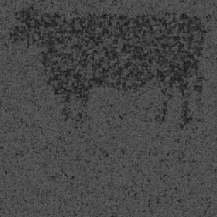
\includegraphics[width=\textwidth, cfbox=black 1pt 0pt]{ress/cow40/cow40.png}}
    %  \vspace{2.0cm}
      \centerline{Noisy image}\medskip
    \end{minipage}
    \hfill
    \begin{minipage}[b]{.30\linewidth}
      \centering
      \centerline{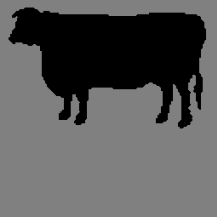
\includegraphics[width=\textwidth, cfbox=black 1pt 0pt]{ress/cow40/cow40_label.png}}
    %  \vspace{1.5cm}
      \centerline{100\% labeled }\medskip
    \end{minipage}
    \hfill
    \begin{minipage}[b]{0.30\linewidth}
      \centering
      \centerline{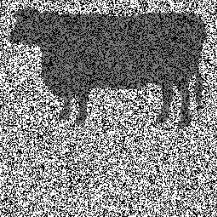
\includegraphics[width=\textwidth,cfbox=black 1pt 0pt]{ress/cow40/cow40_miss.png}}
    %  \vspace{1.5cm}
      \centerline{60\% labeled }\medskip
    \end{minipage}
    \\
    \begin{minipage}[b]{0.30\linewidth}
        \centering
        \centerline{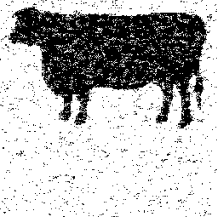
\includegraphics[width=\textwidth,cfbox=black 1pt 0pt]{ress/cow40/cow40_vsl.png}}
      %  \vspace{2.0cm}
        \centerline{VLS (15.64\%)}\medskip      \end{minipage}
      \hfill
      \begin{minipage}[b]{.30\linewidth}
        \centering
        \centerline{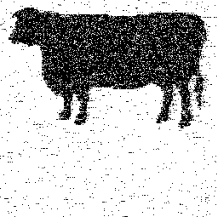
\includegraphics[width=\textwidth,cfbox=black 1pt 0pt]{ress/cow40/cow40_svrnn_2.png}}
      %  \vspace{1.5cm}
        \centerline{SVRNN (16.55\%)}\medskip
      \end{minipage}
      \hfill
      \begin{minipage}[b]{0.30\linewidth}
        \centering
        \centerline{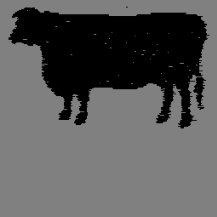
\includegraphics[width=\textwidth,cfbox=black 1pt 0pt]{ress/cow40/cow40_tmm_3.png}}
      %  \vspace{1.5cm}
        \centerline{mTMC (1.93\%)}\medskip
      \end{minipage}
    %
    \caption{Semi-supervised image segmentation with TMC models. }
    \label{fig:res_cow40}
\end{figure}
 
\subsection{Discussion}
\label{subsec:discussion}






\section{Conclusion}
\label{sec:conclusion}
In this paper, we have included some approaches of generatives models 
for semi-supervised learning into a common framework.
We have proposed  a parameter estimation algorithm for TMCs 
based on the variational inference framework and adapted to the
semi-supervised learning setting. 
Our experiments have  shown that a better performance can be 
attained with the mTMC \katy{?? and SVRNN ??models than with the VLS model.
} 



   
% To start a new column (but not a new page) and help balance the last-page
% column length use \vfill\pagebreak.
% -------------------------------------------------------------------------
\vfill
\pagebreak



% References should be produced using the bibtex program from suitable
% BiBTeX files (here: strings, refs, manuals). The IEEEbib.bst bibliography
% style file from IEEE produces unsorted bibliography list.
% -------------------------------------------------------------------------
\bibliographystyle{IEEEbib}
\bibliography{strings,refs}

\end{document}
